% !TeX spellcheck = en_US
\chapter{The IceAct Model in \geant}

\section{\geant}
\geant is a multi-purpose simulation framework for the passage of particles trough matter, written in \textit{C++} and developed by the \geant Collaboration at CERN. It includes physics models, geometry, tracking, hits, and digitization and thus allows a detailed simulation and response analysis for particle detectors in many application fields like particle and accelerator physics, space engineering or medical science. In the framework's source some basic and advanced use cases are implemented and provided as examples. The toolkit is built up of multiple categories (or modules) using each other (cf. figure \ref{geant4:categories}). \cite{geant4}

\begin{wrapfigure}{r}{0.5\textwidth}
	\centering
	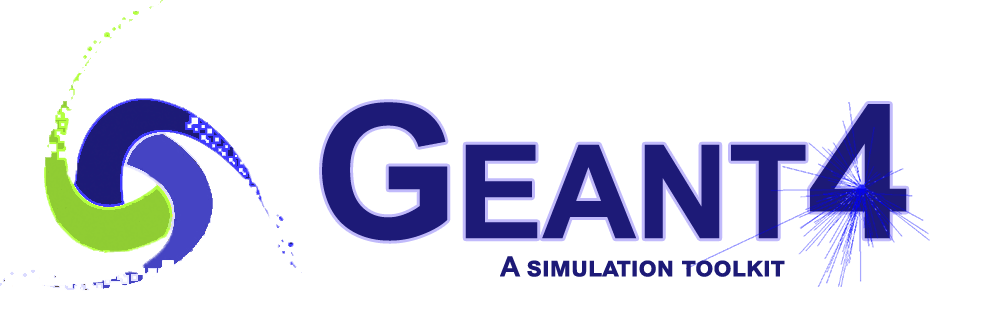
\includegraphics[width=0.5\textwidth]{Geant4Logo.png}
	\caption[\geant Logo]{\textbf{\geant logo.} \cite{geant4:logo}}	
\end{wrapfigure}

\begin{figure}[h]
	\centering
	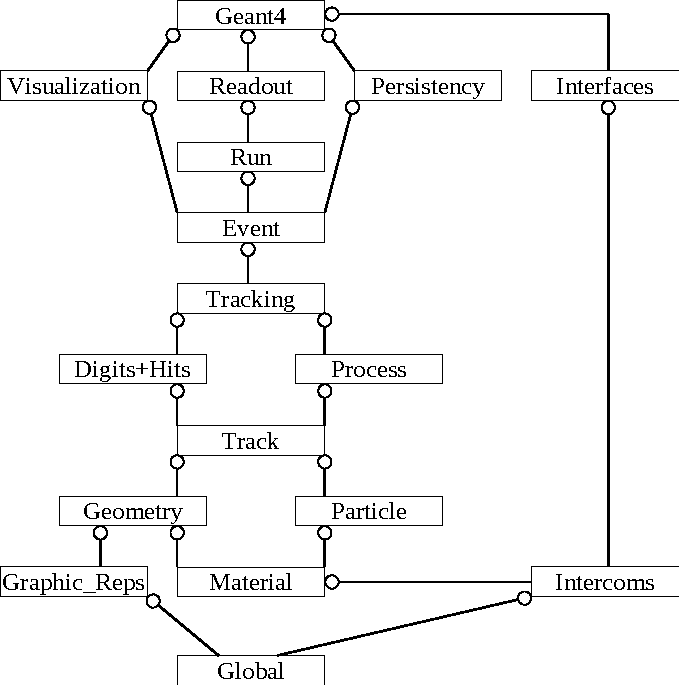
\includegraphics[width=0.5\textwidth]{Geant4ConceptDiagram.pdf}
	\caption[\geant category diagram]{\textbf{Diagram of relationships between \geant categories.} \cite{geant4} The circles represent a \enquote{using} relation. The category with the circle next to the box uses the linked one.}	
	\label{geant4:categories}
\end{figure}

Especially for the use case of IceAct \geant is capable of simulating Cherenkov (optical) photons, material properties like transmission, reflection, and refraction, as well as detection efficiency properties of the SiPMs.

Since this thesis is about an approach of an all-encompassing telescope simulation, \geant provides all major possibilities to get a distinct analysis of the entire optical system of IceAct.

\subsection{FAMOUS telescope simulation}
The fluorescence telescope FAMOUS\footnote{\textbf{F}irst \textbf{A}uger \textbf{M}ulti-pixel
photon counter camera for the \textbf{O}bservation of \textbf{U}ltra-high-energy air \textbf{S}howers} for the Pierre Auger Observatory in Argentina is developed at RWTH Aachen to measure fluorescence light originating from ultra-high-energy cosmic rays (UHECR) by using Silicon Photomultipliers (SiPMs). Withing the development, a detailed \geant simulation has been elaborated. \cite{famous:sim_github,famous:sim_github} The telescope design of FAMOUS is very similar since the detection technique and the optics system is basically the same. Therefore, the IceAct telescope simulation is heavily based on this FAMOUS \geant framework. A detailed discourse and a summary of previous analyses can be found in \cite{famous:niggemann}.

\section{Materials}\label{sec:iceact:model:material}

For an optical device, the material that the light should pass has to be chosen deliberately. Especially the transmission properties, processability, and for IceAct in particular the resistance against harsh weather conditions are of interest.

The glass plate on top of IceAct is made of SCHOTT BOROFLOAT\textsuperscript{\textregistered} 33 borosilicate glass. Borosilicate is chosen for its high durability, transparency in the interesting spectral region, flatness, and weak fluorescence intensities. The refractive index is evaluated at some wavelength. Since we need to have a full dispersion relation the points are spline interpolated (cf. orange curve in figure \ref{iceact:model:material:refractive_index}). \cite{iceact:borosilicate:datasheet}. 

In the data sheet \cite{iceact:borosilicate:datasheet} the transmission properties are given for a vertical light and a glass plate of a thickness of $d = \SI{6.5}{\milli\meter}$. Therefore, the transmission curve $T_\text{total}(\lambda)$ includes the internal absorption as well as the two interface transitions into and out of the borosilicate.
\begin{align}
	T_\text{total}(\lambda) = T_\text{interface}^2(\lambda)\cdot T_\text{internal}(d=\SI{6.5}{\milli\meter},\lambda)
	\label{eq:transmission}
\end{align}
The transmission at the interface can be calculated by using the Fresnel equations. In case of perpendicular light, it is
\begin{align}
	T_\text{interface}(\lambda) = 1 - \left(\frac{n(\lambda)-n_\text{air}}{n(\lambda)+n_\text{air}}\right)^2
	\label{eq:perp_interface_transmission}
\end{align}
In \geant the wavelength dependent absorption length $a(\lambda)$ has to be implemented which is given by the exponential absorption law
\begin{align}
	I(x) = I_0 e^{-\frac{x}{a}} \Leftrightarrow a = - \frac{x}{\ln\left(\frac{I(x)}{I_0}\right)}
	\label{eq:absorptionlaw}
\end{align}
Thus, one gets the absorption length by using equations \eqref{eq:transmission}, \eqref{eq:perp_interface_transmission}, and \eqref{eq:absorptionlaw}.
\begin{align}
	a(\lambda) &= - \frac{d}{\ln T_\text{internal}(d,\lambda)}\\
	&= \frac{d}{2\ln\left(1 - \left(\frac{n(\lambda)-n_\text{air}}{n(\lambda)+n_\text{air}}\right)^2\right)-\ln T_\text{total}(\lambda)}\,,
\end{align}
which is implemented in \geant material properties with $n_\text{air} = 1$. Figure \ref{iceact:model:material:transmission} shows the three transmission components as orange lines.

The Fresnel lens and the Winston Cones in IceAct are made of polymethyl methacrylate (PMMA, acrylic, or plexiglass). The dispersion $n(\lambda)$ can be parametrized with the empirical \textit{Sellmeier equation}. For glasses the usual form is
\begin{align}
	n^2(\lambda) = 1 + \frac{B_1\lambda^2}{\lambda^2-C_1} + \frac{B_2\lambda^2}{\lambda^2-C_2} + \frac{B_3\lambda^2}{\lambda^2-C_3}\,,
	\label{eq:sellmeier}
\end{align}
with the \textit{Sellmeier coefficients} $B_{1,2,3}$ and $C_{1,2,3}$. \cite{iceact:sellmeier} Table \ref{iceact:model:pmma_sellmeiercoeffs} shows the used coefficients and the function is plotted in figure \ref{iceact:model:material:refractive_index} (blue curve).

\begin{table}[h]
	\centering
	\begin{tabular}{c|l}
		$B_1$  & \num{0.99654}  \\
		$B_2$  & \num{0.18964}  \\
		$B_3$  & \num{0.00411}  \\
		$C_1$  & \SI{0.00787}{\micro\meter\squared}  \\
		$C_2$  & \SI{0.02191}{\micro\meter\squared}  \\
		$C_3$  & \SI{3.85727}{\micro\meter\squared}  \\
	\end{tabular}
	\caption[Sellmeier coefficients for PMMA]{\textbf{Sellmeier coefficients for PMMA.} \cite{iceact:refractiveindex} The above-mentioned coefficients are used in the \geant material properties for PMMA. The related Sellmeier equation \eqref{eq:sellmeier} is plotted in figure \ref{iceact:model:material:refractive_index} as the blue curve.}
	\label{iceact:model:pmma_sellmeiercoeffs}
\end{table}

For the transmission properties of PMMA, the same method as for borosilicate is used (see above). Therefore, the data stated in \cite{famous:niggemann} is taken as $T_\text{internal}(d = \SI{3}{\milli\meter})$. Figure \ref{iceact:model:material:transmission} shows the three transmission components as blue lines.

\begin{figure}[h]
	\centering
	\begin{subfigure}[t]{0.485\textwidth}
		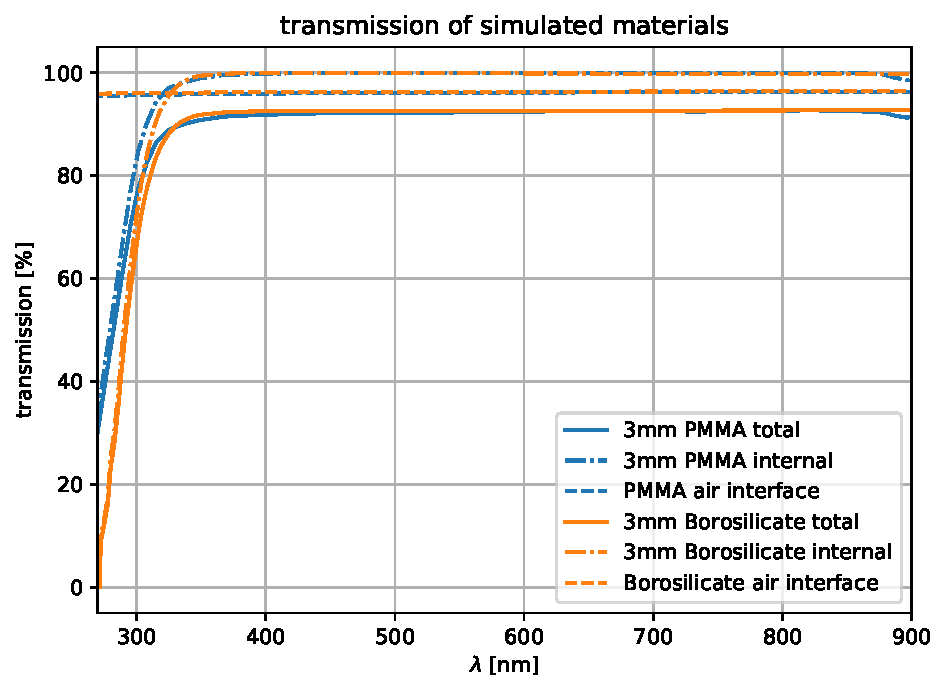
\includegraphics[width=\textwidth]{material/transmission.pdf}
		\caption{full view}
	\end{subfigure}
	\hfill
	\begin{subfigure}[t]{0.499\textwidth}
		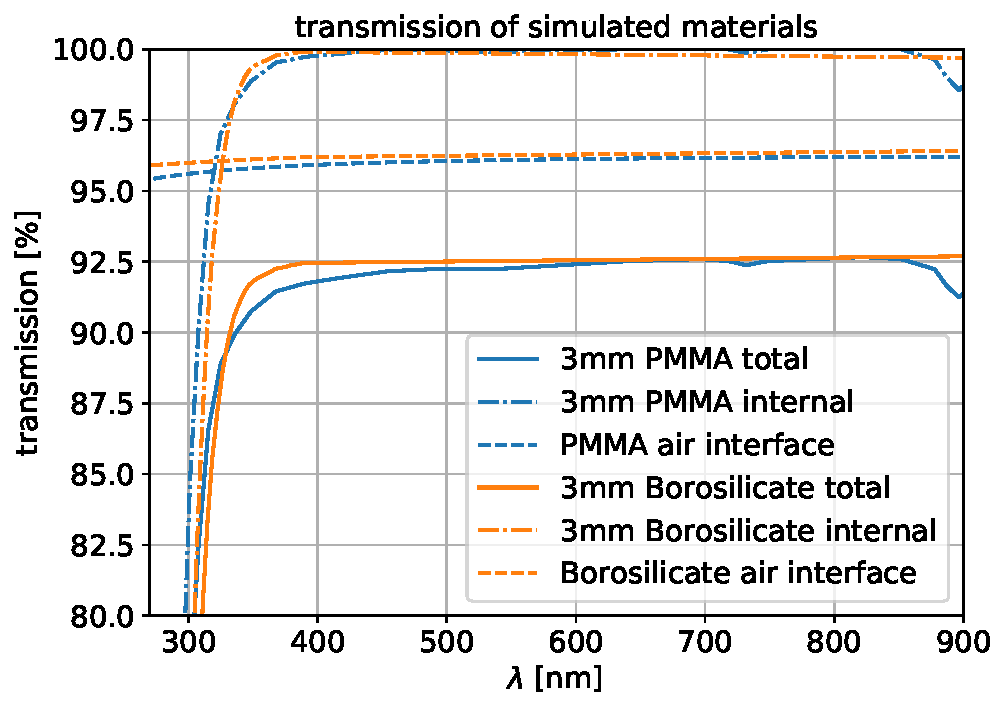
\includegraphics[width=\textwidth]{material/transmission_zoom.pdf}
		\caption{zoomed view}
	\end{subfigure}
	\caption[Transmission of used materials]{\textbf{Transmission functions of materials used in the simulation.} The total transmission function is the product of internal and two interface transmissions which is evaluated for a perpendicularly incident particle in this plot. Thus, the solid lines represent a complete (perpendicular) transition through a \SI{3}{\milli\meter} thick layer of the respective material. For a better comparison, the data of internal transmission for borosilicate is converted from \SI{6.5}{\milli\meter} into \SI{3}{\milli\meter}.}
	\label{iceact:model:material:transmission}	
\end{figure}

\begin{figure}[h]
	\centering
	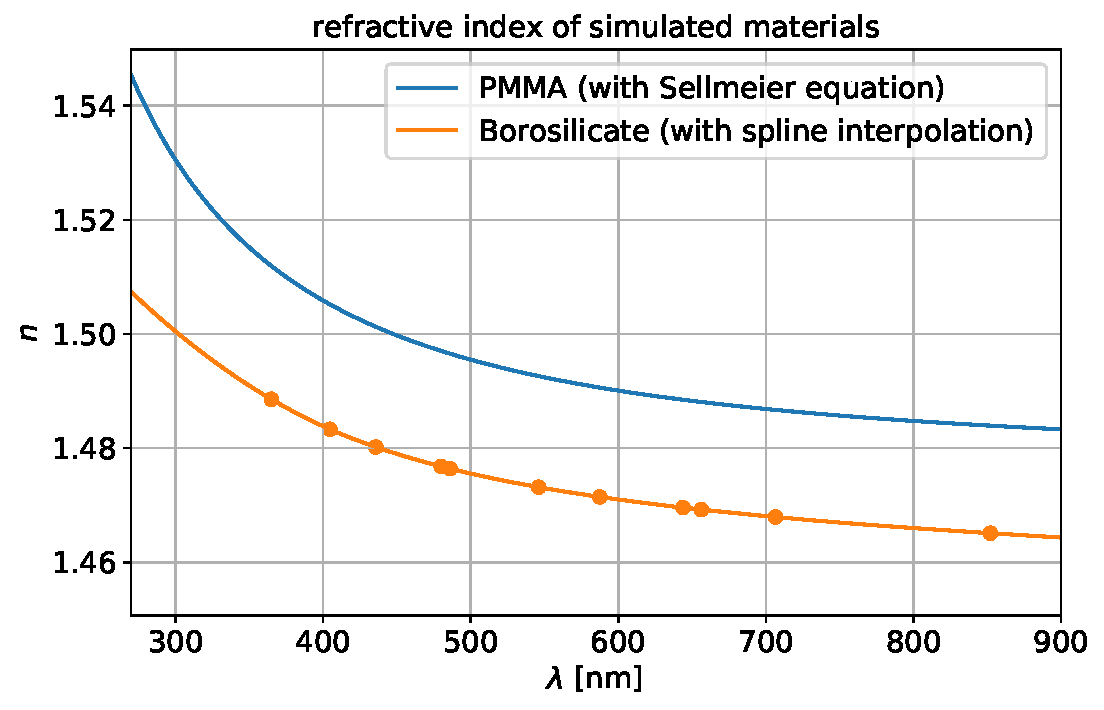
\includegraphics[width=0.7\textwidth]{material/refractive_index.pdf}
	\caption[Refractive index of used materials]{\textbf{Refractive index of materials used in the simulation.} For PMMA the dispersion is calculated by evaluating the Sellmeier equation introduced in this section. The refractive index for the used borosilicate is only given at specific wavelengths. \cite{iceact:borosilicate:datasheet} Therefore, spline interpolation is used to reconstruct the full curve.}
	\label{iceact:model:material:refractive_index}	
\end{figure}

The tube, back plane and other coating surfaces are simulated as \enquote{dummy} material with no reflection or transmission parameters. A particle that hits those surfaces is absorbed and not considered any further.

\section{Optics}

As introduced in section \ref{sec:iceact_intro}, IceAct is designed to image the direction of Cherenkov light on a camera consisting of multiple pixels. The imaging is done by a Fresnel lens, and an SiPM-based camera with light collecting \enquote{cones}. A sketch of the camera layout is shown in figure \ref{iceact:camera:layout}
\begin{figure}[h]
	\centering
	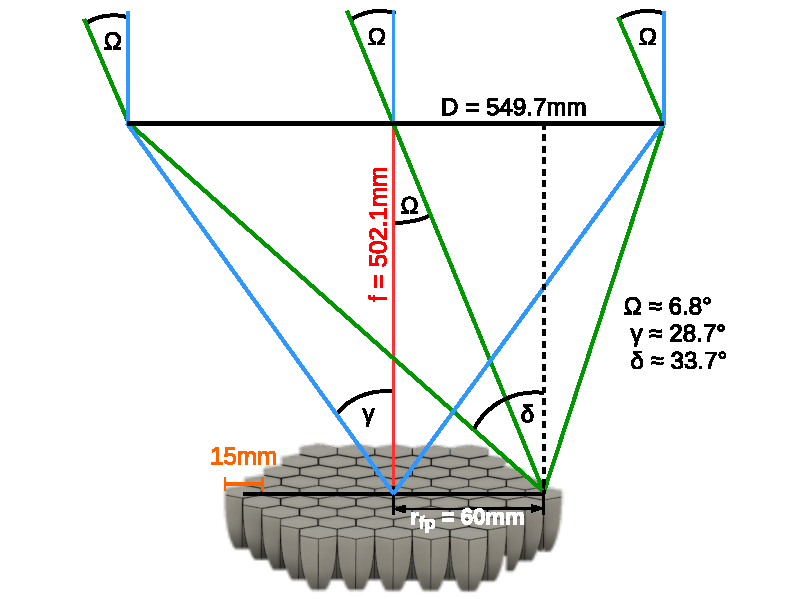
\includegraphics[width=0.6\textwidth]{CameraDesign.pdf}
	\caption[IceAct camera layout]{\textbf{The IceAct camera layout.} \cite{iceact:camera} In this sketch the Fresnel lens with a diameter $D=\SI{549.7}{\milli\meter}$ and a focal length of $f=\SI{502.1}{\milli\meter}$ focusing rays to the camera sketched below. Additionally, three characteristic angles are shown: the maximum incidence angle of a ray to be focused on the camera plane $\Omega\approx\SI{6.8}{\degree}$, the maximum incidence angle on the central Winston cone $\gamma\approx\SI{28.7}{\degree}$, and the maximum incidence angle for the outermost Winston cone $\delta\approx\SI{33.7}{\degree}$.}
	\label{iceact:camera:layout}	
\end{figure}

In the following section the four optical components of the IceAct \geant model are discussed. To have a first glimpse of the model, see figure \ref{iceact:model:cut}.
\begin{figure}[h]
	\centering
	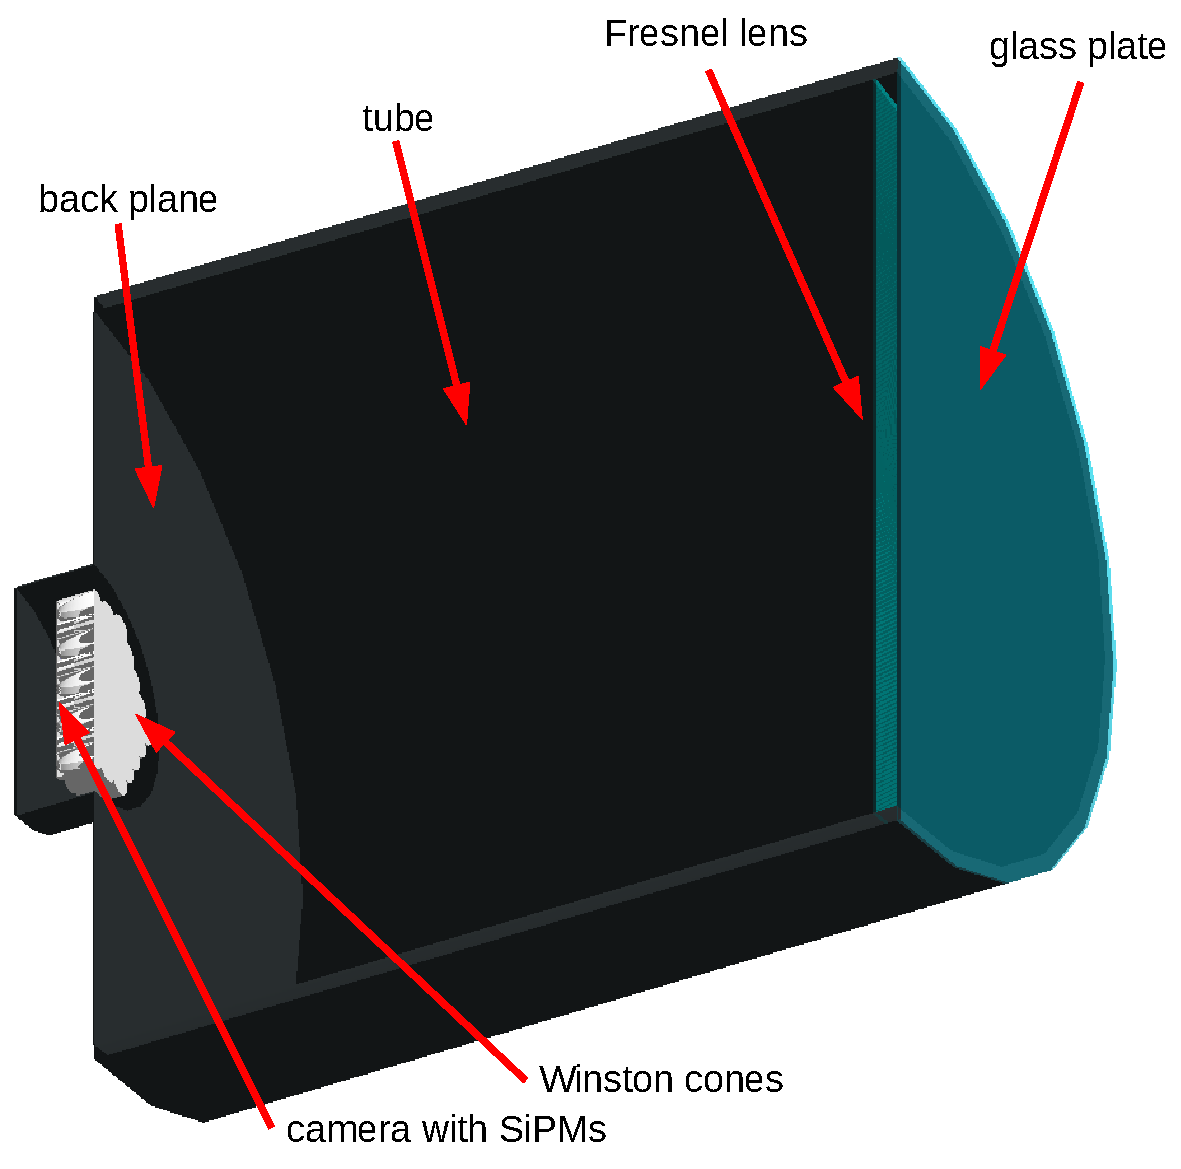
\includegraphics[width=0.6\textwidth]{IceActGeant4Model.pdf}
	\caption[IceAct \geant model]{\textbf{The IceAct \geant model.} Cross-sectional sketch of the IceAct optics in \geant with all simulated components. They are described in detail in \cref{iceact:model:fresnellens,iceact:model:camera,iceact:model:glassplate}.}
	\label{iceact:model:cut}	
\end{figure}

\subsection{Glass Plate}\label{iceact:model:glassplate}

The IceAct glass plate has a thickness of \SI{2+-0.2}{\milli\meter}, a diameter of \SI{650.3+-1}{\milli\meter}, and is made of borosilicate as mentioned in section \ref{sec:iceact:model:material}. It is mounted on top of the tube and its major purpose is to protect the Fresnel lens from the environment. At South Pole conditions, the most challenging for the optical system is adherence of snow above the lens. In the \SI{12.2}{\milli\meter} thick air gap between glass plate and Fresnel lens a heating cable is installed to remove snow from the glass surface. Otherwise, the light would be scattered diffusely at the snow layer and the camera would see a very blurred image.

\subsection{Fresnel Lens}\label{iceact:model:fresnellens}

The two major advantages using a Fresnel lens rather than a conventional lens are the significantly less weight and the fact that light passes less material which could absorb it. The main idea of a Fresnel lens is to divide a thick lens into small annular facets in form of prisms that keep the local inclination of the conventional lens by making local approximations of the lens' \textit{sagitta function}\footnote{In application to lenses, the sagitta function $z(\rho)$ gives the lens thickness $z$ as a function of the radial distance $\rho$ from the optical axis for radially symmetrical lenses.}. Figure \ref{iceact:model:fresnelvsthick} visualizes the principle. IceAct uses the model ORAFOL SC 943 with an aperture of \SI{549.7}{\milli\meter}, a focal length of \SI{502.1}{\milli\meter} at a wavelength of \SI{546+-27.3}{\nano\meter}. The lens is \SI{2.5}{\milli\meter} thick, has 10 grooves per \si{\milli\meter}, and is made of polymethyl methacrylate (PMMA) as stated in section \ref{sec:iceact:model:material}. \cite{iceact:fresnellens:datasheet}

\begin{figure}[h]
	\centering
	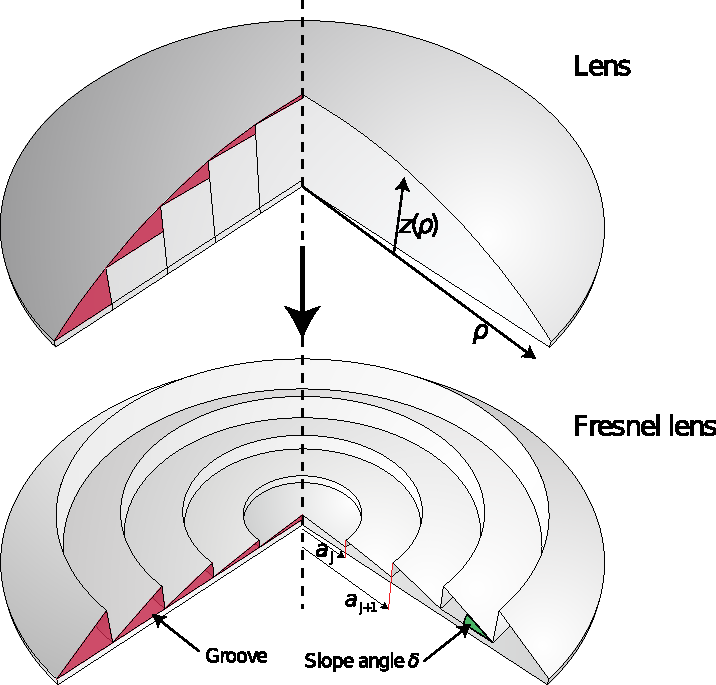
\includegraphics[width=0.5\textwidth]{FresnelVsNormalLens.pdf}
	\caption[Comparison conventional vs. Fresnel lens]{\textbf{Comparison between a conventional \enquote{thick} lens and a Fresnel lens.} \cite{famous:eichler} For the functionality of a lens the radius-dependent sagitta function $z(\rho)$ is crucial. To get rid of the bulky material of a conventional lens, the Fresnel lens is divided into annular \enquote{prisms} called \enquote{grooves}. The slope angle $\delta$ of each groove is a local approximation of the sagitta function to ensure the imaging capability.}
	\label{iceact:model:fresnelvsthick}	
\end{figure}

\begin{figure}[h]
	\centering
	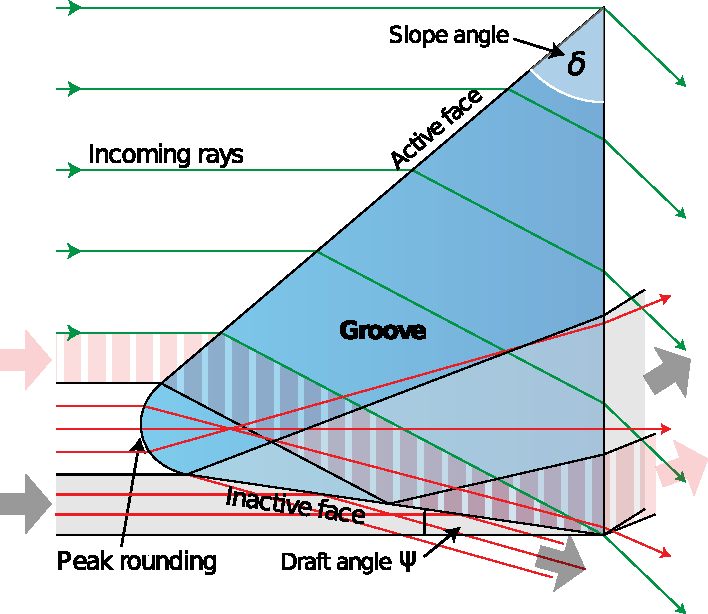
\includegraphics[width=0.5\textwidth]{FresnelGroove.pdf}
	\caption[Fresnel groove]{\textbf{Cross-sectional sketch of a Fresnel groove.} \cite{famous:eichler} Most of the incoming rays are hitting the regular active (or slope) facet of the groove with slope angle $\delta$. For an optimal groove, the inactive (or draft) facet would be parallel to the optical axis. Due to manufacturing process, there is always a small slope on the inactive facet given by the draft angle $\psi$ and the peak is rounded. With this design, there are some impact regions where incoming rays are not refracted to the focal point: if they are total-reflected at the inactive facet inside the groove (red-dashed region), if they hit the peak rounding (red rays), or if they hit the inactive face (gray region).}
	\label{iceact:model:fresnelgroove}	
\end{figure}

\begin{figure}[h]
	\centering
	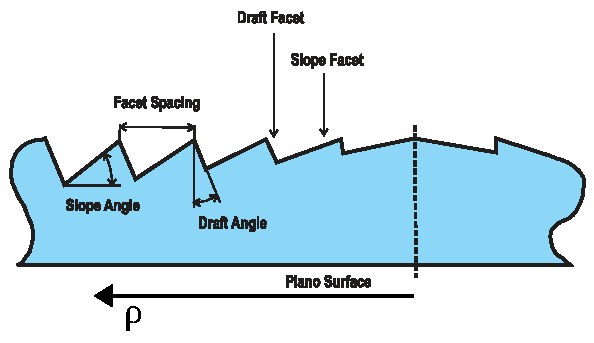
\includegraphics[width=0.5\textwidth]{FresnelSideProfile.pdf}
	\caption[Fresnel side-profile]{\textbf{Side-profile sketch of a Fresnel lens.} \cite[adapted]{iceact:fresnellens:design}. Complementary sketch to figure \ref{iceact:model:fresnelgroove} which shows the manufacturing-driven draft angle increases with radius $\rho$.}
	\label{iceact:model:fresnelprofile}	
\end{figure}

The transmission of a Fresnel lens is not just given by the material properties. Due to the groove structure there are so called \textit{draft facets} where unwanted refractions, reflections, or transmissions occur. One can compensate for this by adjust the \text{draft angle} $\psi$ (cf. figures \ref{iceact:model:fresnelgroove} and \ref{iceact:model:fresnelprofile}) as a function of the lens radius $\rho$. Anyway, the molding process -- which is the common manufacturing technique of Fresnel lenses -- does not allow to have a perpendicular draft facet ($\psi = 0$) due to mold release. This forces the lens to have a minimum draft angle of $\psi_0 = \SI{3}{\degree}$. With the optimization mentioned before, this leads to a radial dependent draft angle which can be expressed as \cite{famous:eichler, famous:niggemann}
\begin{align}
	\psi(\rho) = \SI{3}{\degree} + \SI{0.0473}{\degree\per\milli\meter}\rho\,.
\end{align}
This draft angle function is implemented in the Fresnel lens design in \geant, the groove peak rounding suggested in figure \ref{iceact:model:fresnelgroove} is not.

A detailed discussion and measurement of point spread functions and optical aberrations is done in \cite{famous:niggemann} and \cite{famous:eichler}.

\subsection{Camera}\label{iceact:model:camera}

\begin{figure}
	\centering
	\includegraphics[width=0.6\textwidth]{Camera.png}
	\caption[Picture of an assembled IceAct camera]{\textbf{Picture of an assembled IceAct camera.} \cite{iceact:camera:burgmann} 61 \enquote{hex-to-square} Winston cones are glued onto the hexagonal SiPM grid. Besides, one can see two of the overall three additional pixels for reference measurements.}
	\label{iceact:camera:picture}	
\end{figure}

The IceAct Camera is the compound of 61 Silicon Photomultipliers (SiPMs, cf. section \ref{sec:sipm}) arranged in a hexagonal grid together with 61 Winston cones (cf. section \ref{sec:winstoncones}) glued on them and obviously the readout instrumentation. In addition to the 61 instrumented pixels there are three pixels aside for reference measurements. Two of them are just placed without Winston cones on top to measure optical noise while one pixel is completely \enquote{blind} by being masked. This makes it possible to measure the pure electronic noise of the SiPM. Figure \ref{iceact:camera:picture} shows an assembled IceAct camera. To address each pixel, they are numbered in a spiral scheme starting with the central \enquote{0$\text{th}$} pixel and going outside counterclockwise as seen from the top (cf. figure \ref{iceact:camera:pixelnumbering}).

\begin{figure}[h]
	\centering
	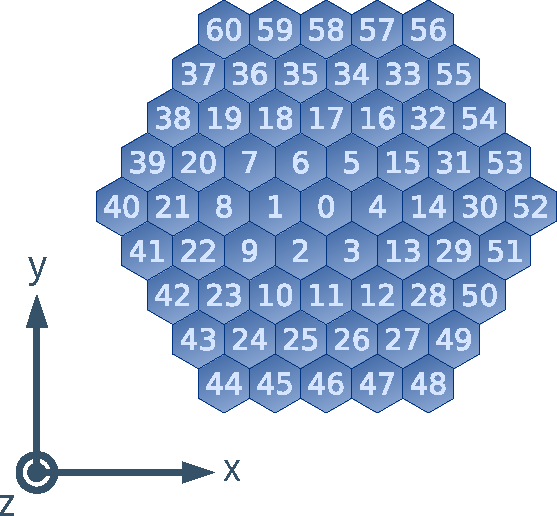
\includegraphics[width=0.4\textwidth]{CameraPixels.pdf}
	\caption[Pixel numbering scheme of the IceAct camera]{\textbf{Pixel numbering scheme of the IceAct camera.} The 61 pixels are numbered in a spiral scheme starting with the central pixel.}
	\label{iceact:camera:pixelnumbering}	
\end{figure}

\todo{technische zeichnung der Kamera mit SiPM abständen}

In the following sections, the working principle as well as the implementation in \geant is discussed.

\subsubsection{Winston Cones}\label{sec:winstoncones}

The IceAct telescopes use a light collection technique to enlarge the detection area of the SiPM grid based on \textit{compound parabolic concentrators} (CPC) \cite{wico:book}. In the following, this concentrators are named \textit{Winston cones}. 
Primarily, a Winston cone is a rotationally symmetrical paraboloid formed by an off-axis parabola revolving around the axis of symmetry (\textit{CPC axis}, cf. figure \ref{iceact:camera:wico_sketch}). Hence, the entrance area $A_\text{en}=\pi a_\text{en}^2$ and the exit area $A_\text{ex}=\pi a_\text{ex}^2$ are circular. The concentration effect works for every ray hitting the entrance area up to the maximum angle $\vartheta_\text{M}$. A relation between $\vartheta_M$ and the characteristic lengths shown in figure \ref{iceact:camera:wico_sketch} can be found: \cite{wico:book,iceact:camera}
\begin{align}
	\sin\vartheta_\text{M} = n\cdot\frac{a_\text{ex}}{a_\text{en}}\,,
	\label{eq:wico:theta_max}
\end{align}
with the refractive index $n$ of the cone material. The appearance of the refractive index connotes the to major working principles of Winston cones. On the one hand, light can be concentrated by using surface reflections in hollow cones ($n=n_\text{air}\approx 1$), or -- on the other hand -- using internal total reflections in solid cones ($n>1$). Equation \eqref{eq:wico:theta_max} shows that the maximum angle can be increased by using a solid cone with a preferably large refractive index.

The parabola describing the Winston cone surface is further called \textit{Winston curve} and can be parameterized by \cite{wico:book,iceact:camera}
\begin{subequations}
	\label{eq:wico:param}
	\begin{align}
	x &= \frac{2a_\text{ex}(1+\sin\vartheta_\text{M})\sin(\phi-\vartheta_\text{M})}{1-\cos\phi}-a_\text{ex}\,,\\
	y &= \frac{2a_\text{ex}(1+\sin\vartheta_\text{M})\cos(\phi-\vartheta_\text{M})}{1-\cos\phi}\,,
	\end{align}
\end{subequations}

with the cone radius $x$, the cone length $y$, and the angle $\phi$ between the connecting line of focus of parabola and a point on the opposite parabola and the parabola axis (cf. figure \ref{iceact:camera:wico_sketch}).

Another important quantity is the cone length $L$ which is given by \cite{wico:book,iceact:camera}
\begin{align}
	L = \frac{a_\text{ex}(1+\sin\vartheta_\text{M})\cos\vartheta_\text{M}}{\sin^2\vartheta_\text{M}}\sim\frac{2a_\text{en}}{2\vartheta_\text{M}}\,.
\end{align}

\begin{figure}
	\centering
	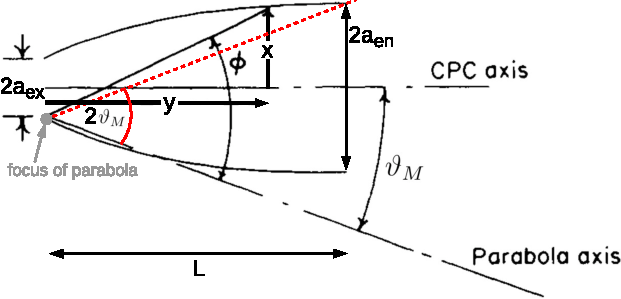
\includegraphics[width=0.6\textwidth]{WinstonConeSketch.pdf}
	\caption[Sketch of a Winston cone]{\textbf{Sketch of a Winston cone.} \cite{iceact:camera} The shape of the cone is given by the two sketched parabolic curves rotating around the CPC axis. Characteristic lengths and angles are indicated: the entrance and exit diameters $a_\text{en,ex}$, the cone length $L$, the maximum incidence angle $\vartheta_\text{M}$, the parameterization coordinates $(x,y)$, and the angle $\phi\in[\vartheta_\text{M},\vartheta_M+\SI{90}{\degree}]$ needed for parameterization as well.}
	\label{iceact:camera:wico_sketch}	
\end{figure}

By appropriate design, Winston cones fulfill all requirements for light concentrators in IceAct given by the optical layout (cf. figure \ref{iceact:camera:layout}).
However, one can design an improved Winston cone for the purposes in IceAct since a hexagonal grid of quadratic pixels with an area of $\SI{6}{\milli\meter}\times\SI{6}{\milli\meter}$ is used \todo{referenz zur techn. Zeichnung der Kamera}. Instead of a radially symmetrical cone, the IceAct Winston cone is designed in such a way that the exit window fits the SiPM area while the entrance window is hexagonal to maximize the camera's detectional area (cf. figure \ref{iceact:camera:picture}). This design is called \textit{hex-to-square}. A sketch of the IceAct Winston cone is shown in figure \ref{iceact:camera:iceact_wico_sketch}. In it, one can see a green dashed line and a pink solid line on the cone's side which follow optimized Winston curves by using the parameterization of equations \eqref{eq:wico:param}.

\begin{figure}
	\centering
	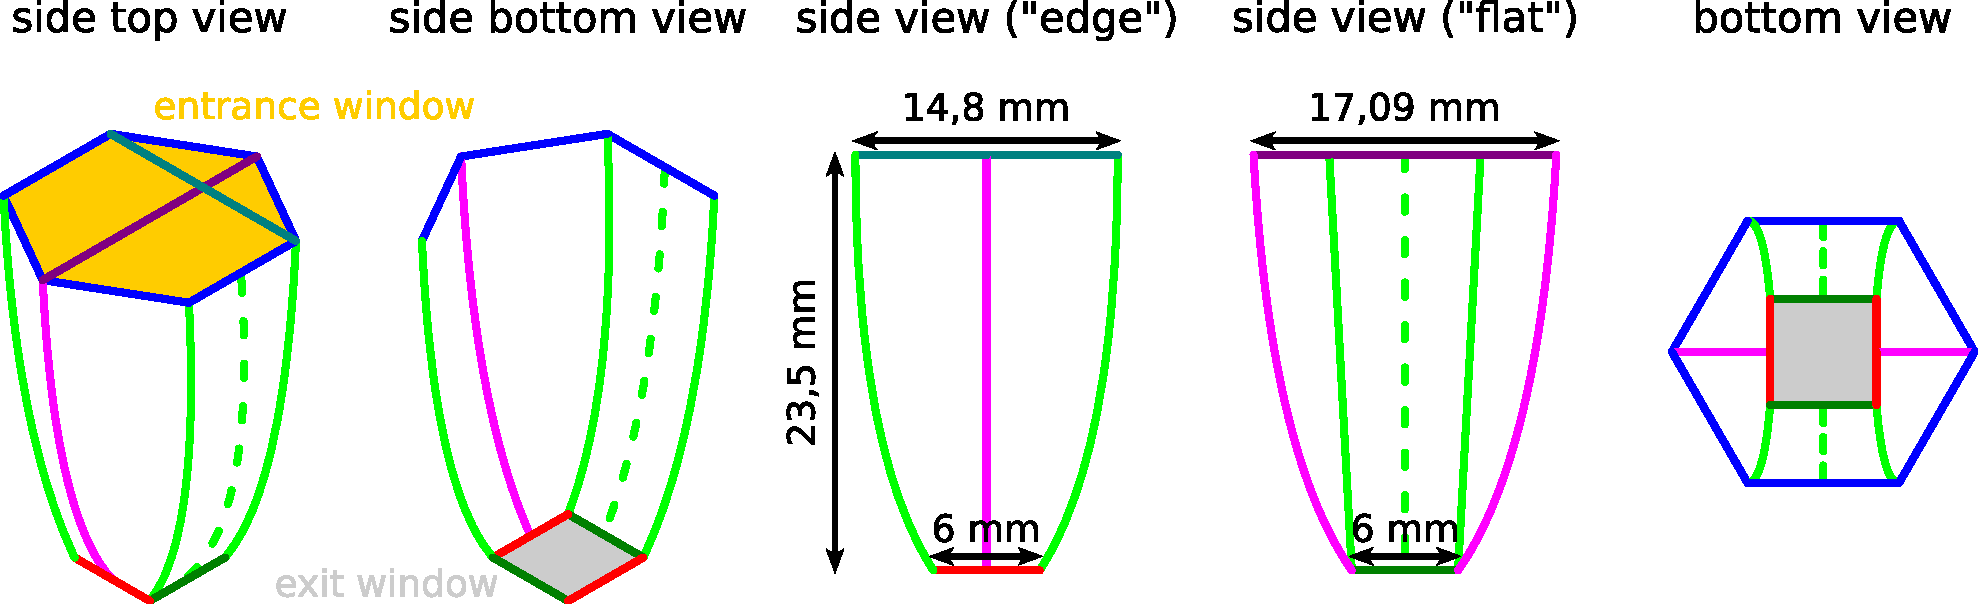
\includegraphics[width=\textwidth]{IceActWiCoSketches.pdf}
	\caption[Sketches of the IceAct \enquote{hex-to-square} Winston cone]{\textbf{Sketches of the IceAct \enquote{hex-to-square} Winston cone.} The cone is shown from different points of view with dimensioning. The pink edge and the green dashed surface line follow the optimized Winston curve functions developed in \cite{iceact:camera}. The green dashed curve is extruded in order to form the whole side. Two different functions result in two different maximum angles $\vartheta_\text{M}^\text{edge,side}$ for an incidence parallel to the \enquote{edge} or the \enquote{side} plane.}
	\label{iceact:camera:iceact_wico_sketch}	
\end{figure}

Hence, the application of Winston cones extend the detectional area of the pixels by a factor of (cf. figure \ref{iceact:camera:iceact_wico_sketch})
\begin{align}
	\frac{A_\text{camera with WiCos}}{A_\text{camera without WiCos}} = \frac{61\cdot \frac{3}{2}\sqrt{3}\cdot\left(\frac{\SI{17.09}{\milli\meter}}{2}\right)^2}{61\cdot(\SI{6}{\milli\meter})^2}\approx\num{5.27}\,.
\end{align}

Due to its complex shape the cones are implemented in \geant by decomposing their CAD\footnote{\textbf{C}omputer-\textbf{a}ided \textbf{D}esign, technique to use a computer for the creation, analysis, etc. of a design.} sketch into small triangular tiles called \textit{meshgrid}. This meshed geometry is then translated into \geant by using the toolkit \textit{CADMesh} \cite{wico:cadmesh}. More about Winston cone meshing is discussed in section \ref{sec:wico_meshing}.

\subsubsection{Silicon Photomultipliers}\label{sec:sipm}

Silicon Photomultipliers (\textit{SiPM}s) are compact devices used for photon detection in multiple applications. 

\todo{write}

